\documentclass[a4paper,10pt]{article}
\usepackage[utf8x]{inputenc}
\usepackage{array}
\usepackage{graphicx}
\usepackage{float}
\usepackage{color}
\usepackage{alltt}
\usepackage[T1]{fontenc}
\usepackage{ae,aecompl}

%opening
\title{Generalized Top Down Parsing In Cubic Time}
\author{Arnold Lankamp}

\begin{document}

\maketitle

\begin{abstract}

In this article we will describe our generalized top down parsing algorithm. Since it's top-down it will be easier for a human to understand. Additionally we will also demonstrate that, in terms of efficiency, our implementation performs excellent.

TODO: We need some more text here.

\end{abstract}

\section{Introduction}

If the abstract didn't catch your attention yet, here are some highlights:
\begin{itemize}
 \setlength{\itemsep}{0pt}
 \setlength{\parskip}{0pt}
 \setlength{\parsep}{0pt}

 \item Worst-case cubic space and time bounds with respect to the length of the input string.
 \item Worst-case linear scaling relative to the size of the grammar.
 \item Linear performance on LL(k) and LR(k) grammars.
 \item No significant performance hit for rules that are not left factored.
 \item Generating or hand crafting the recognizer / parser code is trivial.
 \item Parse traces are easy to follow; using a debugger to step through the parse process can actually be informative.
 \item Low constant overhead.
\end{itemize}
We call our parser, the Scannerless Binary Forest Generalized Top Down Parser or SBFGTD (BF also means Bloody Fast, in case your wondering why it was put in the abbreviation).

TODO: Motivation.\\
-Easier to comprehend, since it's top-down; which is more in-line with human thinking. (Why do we want this?)\\
-Top-down is considered to be too slow in general, so it's fairly unpopular.

\section{Recognizer}

First we will discuss the algorithm for the recognizer, for simplicity's sake. Further on in this article we will explain how the recognizer can be extended to become a parser.

\subsection{GSS}

As is common in generalized parsing, we use a kind of Graph Structured Stack (GSS). In our case we generate a stack node with a unique identifier for every item in the grammar. For example; if take the following grammar: $S\,::=\,AB\,|\,BA,\,A\,::=\,a,\,B\,::=\,b$, we would assign these identifiers as follows: $.S$(-1), $.AB$(0), $A.B$(1), $.BA$(2), $B.A$(3), $.a$(4) and $.b$(5). These identifiers are needed to be able to handle the sharing of GSS nodes correctly, so regardless whether or not comparable items exist, they should not be merged. Each stack node consists of this identifier, edges back to their 'parents' in the graph and information about its 'right neighbour' in the production, so we know where to go next.

\subsection{Basic algorithm}

\begin{enumerate}
 \setlength{\itemsep}{0pt}
 \setlength{\parskip}{0pt}
 \setlength{\parsep}{0pt}

 \item Expand the left most node of every production that did not match anything yet on all stacks, until no stacks can be expanded anymore (i.e. they all have a terminal at the bottom).
 \item Match all nodes on the bottom of the stacks to the input. Reduce the ones that match, remove the ones that don't.
 \item Reduce the nodes on all stacks that matched something and have them queue the 'next' node in the production they are part of where applicable, until no reductions are possible anymore.
 \item If there are nodes queued for expansion go to 1.
 \item If the end of the input has been reached and we have at least one derivation for one of the start symbols we are successful; otherwise recognizing failed.
\end{enumerate}

\subsection{Pseudocode}

{\small
\begin{verbatim}
parse(){
  toExpandSet.add('startNode');
  expand();
  
  do{
    reduce();
    expand();
  }while(toReduceSet.notEmpty());
  
  if(endOfInputHasNotBeenReached()) error;
}
\end{verbatim}
}

This is the main loop of the recognizer. It alternates between expanding and reducing, until there is nothing left to be done. Once we exit the loop we check whether or not we reached the end of the input. If we did, we recognized at least one complete derivation and are thus successful, otherwise we encountered an error.

{\small
\begin{verbatim}
expand(){
  while(toExpandSet.notEmpty()){
    node = toExpandSet.pop();
    
    Node[] children = getChildrenFor(node);
    for(childNode <- children){
      if(reducedStore.contains(childNode)){ // Child already has results
         if(toReduceSet.notContains(node)){ // Sharing
           toReduceSet.add(node);
         }
      }else{
        if(childNode.isTerminal()){
            toReduceSet.add(childNode);
        }else{
          if(expandedStore.contains(childNode)){ // Sharing
            expandedStore.get(childNode).addEdge(node);
          }else{
            toExpandSet.add(childNode);
            
            expandedStore.add(childNode);
          }
        }
      }
    }
  }
}
\end{verbatim}
}

This is the expand loop of the recognizer. We take one node from the {\bf toExpandSet} and add its non-terminal 'children' to the {\bf toExpandSet}, in case they haven't been expanded or been queued for expansion before; nodes that have been expanded before will be in the {\bf expandedStore}. And its terminal 'children' to the {\bf toReduceSet}. The exception to this is, when we encounter a 'child' that already has been reduced; which we check by looking in the {\bf reducedStore}. If this is the case we queue the node we are currently handling for reduction by putting it in the {\bf toReduceSet} (if not done so already). We keep iterating until the {\bf toExpandSet} is empty.

Note that the 'stores' need to be implemented as an array or table that has a set of non-terminals associated with every index in the input string (with O(1) look-up time). Otherwise it is not possible to guarantee worst-case cubic time complexity.

{\small
\begin{verbatim}
reduce(){
  while(toReduceSet.notEmpty()){
    node = toReduceSet.pop();
    reducedStore.add(node);
    
    if(node.isTerminal() && !node.matches()) continue;
    
    if(node.lastInProduction()){
      for(parent <- node.edges){
        if(toReduceSet.notContains(parent) &&
            reducedStore.notContains(parent)){ // Sharing (is reduced)
          toReduceSet.add(parent);
        }
      }
    }else if(node.hasNext()){
      next = node.next;
      if(toExpand.contains(next)){ // Sharing
        next = toExpandSet.get(next);
      }else if(expandedStore.notContains(next)){ // Sharing
        toExpandSet.add(next);
      }
      next.addEdges(node.edges);
    }
  }
}
\end{verbatim}
}

TODO: Explain.

\subsection{Correctness}

TODO: Prove.\\
-Conceptually easy to get your head around.\\
-Discuss terminalization of left-recursive rules.

\subsection{From grammar to code}

Converting a grammar to a recognizer or parser, either by hand writing or generating it, is relatively straight forward. All that is needed is a direct translation from the grammar rules to either functions or some kind of table like data structure. Basically it just needs to know what alternatives are associated with a each left-hand-side. In case we are generating code, this would mean that we need one function per non-terminal, which contains logic that informs the recognizer about what alternatives should be expected.

Since the mapping between the original grammar and the code or table is one-on-one, it is possible to implement or edit it by hand without much effort. Another advantage is that, in combination with the top-down-ness of our algorithm, it makes tracing errors in a grammar easier; if you'd want to know why something doesn't match at a certain position, you can just go through it with a debugger to see what happens. Your degree of success naturally depends on the amount of stacks that are alive at the moment you're trying to observe, but at least the possibility to do so exists.

\subsection{Example traces}

To illustrate how the recognizer works, here are some example traces.

\subsubsection{Straight forward}
$S\,::=\,AB$\\
$A\,::=\,a$\\
$B\,::=\,b$\\
input = $ab$

\begin{enumerate}
 \setlength{\itemsep}{0pt}
 \setlength{\parskip}{0pt}
 \setlength{\parsep}{0pt}
 
 \item expand $.S$
 \item expect $.AB$
 \item expand $.AB$
 \item expect $.a$
 \item reduce $a.$ and follow edge to $.AB$
 \item move from $.AB$ to $A.B$
 \item expand $A.B$
 \item expect $.b$
 \item reduce $b.$ follow edge to $A.B$
 \item reduce $AB.$ and follow edge to $.S$
 \item reduce $S.$
 \item done.
\end{enumerate}

\subsubsection{Left recursive}
$S\,::=\,A$\\
$A\,::=\,Aa\,|\,a$\\
input = $aaa$

\begin{enumerate}
 \setlength{\itemsep}{0pt}
 \setlength{\parskip}{0pt}
 \setlength{\parsep}{0pt}
 
 \item expand $.S$
 \item expect $.A$
 \item expand $.A$
 \item expect $.Aa$ $|$ $.a$
 \item expand $.A$ $\Rightarrow$ $.A$ shared
 \item reduce $a.$ and follow edges to $.S$ and $.Aa$
 \item parse for $S.$ is incomplete and is discarded
 \item move from $.Aa$ to $A.a$
 \item reduce $Aa.$ and follow edges to $.S$ and $.Aa$
 \item parse for $S.$ is incomplete and is discarded
 \item move from $.Aa$ to $A.a$
 \item reduce $Aa.$ and follow edges to $.S$ and $.Aa$
 \item parse for $S.$ is complete.
 \item move from $.Aa$ to $A.a$
 \item reduce $Aa.$ failed, since EOI has already been reached.
 \item done.
\end{enumerate}

TODO: Maybe convert to illustrations?\\
TODO: Add some text around it.

\subsection{Worst-case complexity}

Since the GSS only contains nodes that we expect to 'encounter', there are at most $O(N)$ of them; where $N$ is the number of characters in the input string. Each node only has one edge to each of it's possible parents per level and there are $N$ levels, there are at most $O(N)$ edges per node. In the worst-case there are $N$ times $O(N)$ nodes that match a substring that ends at the 'current' level. When moving to the 'next' node in the production, all edges of these nodes need to be carried over. Since these sets of edges need to be merged, the time this operation needs to complete is equal to the number of levels before (and including) the 'current' level (so $N$ at most). This means that the total algorithm becomes $O(N^3)$ worst-case.

Reducing consumes $O(N^2)$ time at most in the worst-case, since each of the $O(N^2)$ edges will only be followed once and the check whether or not each of the 'parents' still needs to be reduced, is an operation that completes in $O(1)$ time.

\section{Parser}

\subsection{Parse forest}

To represent the parse forest we use a format that was especially designed for this parser, to ensure worst-case behaviour remains within cubic time and space bounds. We call it 'deflattenized', for lack of a better description; it's intent is similar to binarization, but it's implementation is somewhat different.

The parse forest consists of nodes. Every node in the forest contains a result, which represents a substring for a certain symbol. In case this symbol is a non-terminal, this result contain one or more references to alternative representations of the substring it denotes. Each node also contains a set of prefixes. A prefix only consists of a reference to a node. If you trace all possible paths through this representation of a production to the start, you'll get all alternatives for a this production at a certain location.

\subsubsection{Example}
To give an idea of what a typical parse forest would look like we will give an example using the following grammar:\\
$S\,::=\,AAA$\\
$A\,::=\,a\,|\,aa$\\
input = $aaaa$

\begin{figure}[H]
\centering
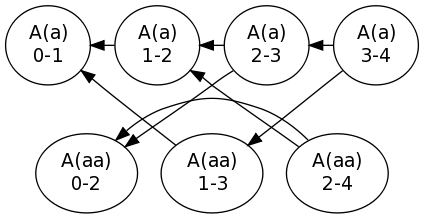
\includegraphics[width=0.5\textwidth]{a_aa-forest.png}
\caption{A visual representation of the parse forest, showing all alternatives for the four character input string. The numbers indicate the start and end position of the matched substring.}
\end{figure}

In the figure above we see the parse forest. It illustrates how the parse results are stored in memory.

To show how we can obtain all possible derivations from this parse forest, we will list them in the table below; which relates each path through the forest to a derivation.

\begin{table}[H]
\centering
\begin{tabular}{ p{15em} p{15em} }
Derivation & Forest path\\
\hline
S(A+(A(a),A(a),A(aa))) & $A0$-$1$ $\leftarrow$ $A1$-$2$ $\leftarrow$ $A2$-$4$\\
S(A+(A(a),A(aa),A(a))) & $A0$-$1$ $\leftarrow$ $A1$-$3$ $\leftarrow$ $A3$-$4$\\
S(A+(A(aa),A(a),A(a))) & $A0$-$2$ $\leftarrow$ $A2$-$3$ $\leftarrow$ $A3$-$4$
\end{tabular}
\caption{'Flattened' version of the parse forest}
\end{table}

\subsection{Psuedocode}

Augmenting our recognizer with parse tree construction code is trivial. Only a few minor adjustments are needed. Additions are highlighted in italic.

{\small
\begin{alltt}
parse()\{
  toExpandSet.add('startNode');
  expand();
  
  do\{
    reduce();
    expand();
  \}while(toReduceSet.notEmpty());
  
  if(endOfInputHasNotBeenReached()) error;
  \textit{
  return findResultStore('startNode');}
\}
\end{alltt}
}

TODO: Explain changes.

{\small
\begin{alltt}
expand()\{
  while(toExpandSet.notEmpty())\{
    node = toExpandSet.pop();
    
    Node[] children = getChildrenFor(node);
    for(childNode <- children)\{
      if(reducedStore.contains(childNode))\{\textit{
        findResultStore(node).
            addAlternative(childNode.prefixes, childNode.results);}
        if(toReduceSet.notContains(node))\{ // Sharing
          toReduceSet.add(node);
        \}
      \}else\{
        if(childNode.isTerminal())\{
            toReduceSet.add(childNode);
        \}else\{
          if(expandedStore.contains(childNode))\{ // Sharing
            expandedStore.get(childNode).addEdge(node);
          \}else\{
            toExpandSet.add(childNode);
            
            expandedStore.add(childNode);
          \}
        \}
      \}
    \}
  \}
\}
\end{alltt}
}

TODO: Explain changes.

{\small
\begin{alltt}
reduce()\{
  while(toReduceSet.notEmpty())\{
    node = toReduceSet.pop();
    reducedStore.add(node);
    
    if(node.isTerminal() && !node.matches()) continue;
    
    if(node.lastInProduction())\{
      for(parent <- node.edges)\{\textit{
        findResultStore(parent).
            addAlternative(node.prefixes, node.results);}
        if(toReduceSet.notContains(parent) &&
            reducedStore.notContains(parent))\{ // Sharing (is reduced)
          toReduceSet.add(parent);
        \}
      \}
    \}else if(node.hasNext())\{
      next = node.next;
      if(toExpandSet.contains(next))\{ // Sharing
        next = toExpandSet.get(next);
      \}else if(expandedStore.notContains(next))\{ // Sharing
        toExpandSet.add(next);
      \}
      next.addEdges(node.edges);\textit{
      next.updatePrefixes(node.prefixes, node.results);}
    \}
  \}
\}
\end{alltt}
}

TODO: Explain changes.

{\small
\begin{alltt}
\textit{findResultStore(node)\{
  return resultStores.
    findOrCreate(node.startLocation, node.endLocation, node.name);
\}}
\end{alltt}
}

TODO: Explain.

\subsection{Correctness}

TODO: Prove.\\
-Hidden right recursion is problematic, but handled correctly by our implementation; the rest is fairly obvious.

\subsection{Worst-case complexity}
Every node in the tree is identified by the substring its contained result represents and its prefixes. There can be only one result per substring, this means there are at most $O(N^2)$ results. The prefix sets are identified by the start and end position of the substring they represent, so there are at most $O(N^2)$ of them. Each prefix set can contain up to $N$ different prefixes, which all denote the same substring; at most one per location (before the current location) in the input string. The number of unique nodes is determined by multiplying the number of results by the number of prefix sets. However, since a prefix set can only be matched in a node, together with a result that starts at the same position as the prefix ends each prefix set can be associated with $O(N)$ different nodes at most. Hence the number of unique nodes is limited to $O(N^3)$, making the parse forest $O(N^3)$ worst-case. Note that in the implementation all prefix sets are shared regardless of the end position of the node they are matched to, to improve efficiency; this has no effect on worst-case behaviour, but does improve performance and memory usage in the general case.

\subsubsection{Flattening}
Optionally it is possible to output a flattened version of the parse forest at the user's request. Naturally this parse forest will be unbound polynomial in size in the worst-case. In practice this unlikely to happen; moreso since filtering can be done during parsing and flattening, making it improbable that many ambiguities remain in the final tree, in the general case. We'll discuss filtering later on in this document.

\subsubsection{Worst-case example}
We've already theoreticly proven that the parse forest will be $O(N^3)$ in the worst-case. In this section we will show that in practice this is indeed the case.

Here is an overview of the parse forest's statistics for the following grammar:\\
$S\,::=\,SSS\,|\,SS\,|\,a\,|\,\epsilon$\\
input = $a * 1$ to $a * 10$, $a * 50$, $a * 100$, $a * 200$, $a * 300$, $a * 400$ and $a * 500$

\begin{table}[H]
\centering
\begin{tabular}{ | p{6em} | p{4em} | p{5em} | p{4em} | p{5em} | }
  \hline
  Input length & Results & Prefix sets & Nodes & Nodes / $N^3$ \\
  \hline
  0 & 1 & 2 & 2 & - \\
  1 & 4 & 6 & 6 & 6 \\
  2 & 7 & 12 & 13 & 1.625 \\
  3 & 11 & 20 & 24 & 0.889 \\
  4 & 16 & 30 & 40 & 0.625 \\
  5 & 22 & 42 & 62 & 0.496 \\
  6 & 29 & 56 & 91 & 0.421 \\
  7 & 37 & 72 & 128 & 0.373 \\
  8 & 46 & 90 & 174 & 0.34 \\
  9 & 56 & 110 & 230 & 0.316 \\
  10 & 67 & 132 & 297 & 0.297 \\
  \hline
  50 & 1327 & 2652 & 23477 & 0.188 \\
  100 & 5152 & 10302 & 176952 & 0.177 \\
  200 & 20302 & 40602 & 1373902 & 0.172 \\
  300 & 45452 & 90902 & 4590852 & 0.170 \\
  400 & 80602 & 161202 & 10827802 & 0.169 \\
  500 & 125752 & 251502 & 21084752 & 0.169 \\
  \hline
\end{tabular}
\caption{Worst-case parse tree data}
\end{table}

In the table above we can see how the different components in the parse forest increase with respect to the length of the input string. The number of results increases by $N + 1$ for every extra character in the input string. The number of prefix sets scales in a similar way, although there are roughly twice as many of them in comparison to results, since both the second and the third $S$ in $SSS$ need a prefix. As can be observed, the number of nodes remains within cubic bounds for this worst-case example.

\section{Extended capabilities}

To improve the usefulness of the parser on real grammar a few additions were made. Namely support for lists, optionals and certain non-context-free features is added. In this chapter we will discuss their implementation.

\subsection{Lists}

List, separated lists and optionals are handled in a similar way, because in essense they are the same. However their semantics are slightly different; separated lists are lists with extra symbols between their elements and optionals are star-lists with one element at most; from here on out we will refer to all of these simply as 'lists'.

Often lists are implemented by adding extra 'virtual' rules to the grammar. For example $S\,::=\,A+,\,A\,::=\,a$ can be parsed like a 'normal' grammar, if we add the rule $A+\,::=\,AA+\,|\,A$. The advantage of this approach is that the parser does not need to be modified. On the other hand, we always get a binarized version of the list as a result, that uses these imaginary productions, which may not be what we wanted. Additionally, because an extra rule is inserted into the grammar we need more GSS nodes to be able to parse the list.

Our approach involves special casing the handling of lists, by introducing additional types of GSS nodes that contain knowledge about how they need to be expanded. For example to expand the star-list $A*$, it would queue an $\epsilon$ and a $A$ non-terminal GSS node; this $A$ GSS node has a 'next' point to itself and is marked as last node in the 'production' (see figure below). One could view this construction as a GSS node with a kind of dynamicaly growing production as its child. Each time an $A$ is recognized the list is reduced and the next $A$ is pushed on the stack to be recognized; causing the next element to be appended to the list.

\begin{figure}[H]
\centering
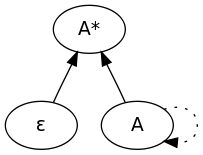
\includegraphics[scale=0.5]{star-list.png}
\caption{GSS representation of a expanded star-list; the solid arrows represent edges and the dotted arrows 'next pointers'.}
\end{figure}

These list children can be shared just like any other GSS node. Nothing special needs to be done for this. Since this is the case, worst-case time and space bounds do not change by the introduction of this feature.

Exactly the same principle is used for separated lists and optionals. We won't go into detail on those, since one can easily imagine how those work.

\subsection{Location}

Similar to how lists are implemented, there are also specialized GSS nodes for location related indicators. We have the following varieties:
\begin{enumerate}
 \setlength{\itemsep}{0pt}
 \setlength{\parskip}{0pt}
 \setlength{\parsep}{0pt}
 
 \item Start-of-line
 \item End-of-line
 \item At-column($X$); where $X$ indicates the column number
\end{enumerate}
Basically these are epsilons that only match when we are at a specific location in the input. So they don't consume input and they are not context free. However they can be useful when parsing certain languages nonetheless.

\section{Optimizations}

The basic algorithm is fairly straight forward and relatively simple to implement. The naïve implementation will respect worst-case cubic time and space bounds, however adaptations can be made to improve its overall efficiency.

\subsection{General}

\subsubsection{Breadth-first}
Making the implementation breadth first generally reduces resource usage. This is because it enables us to determine when certain data is no longer necessary and can be discarded. Additionally, since most information is stored on a per-level basis, we can exploit the assumption that we are level synchronized to our advantage. For example, the memory used for stacks that died off can be reclaimed and reused and sharing and such can be handled slightly more efficiently.

\subsubsection{Matching}
Another minor performance improvement can be made by matching on entire literals at once, instead of on characters. This decreases the amount of necessary GSS nodes and thus reduces stack activity.

\subsubsection{Look-ahead}
A more obvious optimization is adding support for look-ahead filtering. Simply by adding simple checks to the (generated) parser code, we can prevent unnecessary work; if a certain alternative will never match, we don't need to expect it. The number of characters we look ahead is not limited by theoretical or practical constraints.

\subsection{Edge related}

Generally parsers store results on edges in the GSS. If we would refrain from doing this and store parse results elsewhere (in a table with constant look-up time), edges could remain pointers. At first sight this may not be an advantage, however we would be able to share edges among GSS nodes and it opens up numereous other interesting opportunities for optimization.

\subsubsection{Expansion}
First of all, by caching 'expected children' for every type of node per level a substantial performance increase can be achieved. Namely, this will ensure linear scaling for non-left-factored grammars. The reason for this is the following; for example, if we take the grammar rules:\\
$S\,::=\,E$\\
$E\,::=\,E + E\,|\,E - E$.\\
The expansion at the first level would look like this:
\begin{enumerate}
 \setlength{\itemsep}{0pt}
 \setlength{\parskip}{0pt}
 \setlength{\parsep}{0pt}
 
 \item $.E$ $\rightarrow$ $.E+E$
 \item $.E+E$ edges = \{$.E$\}
 \item $.E$ $\rightarrow$ $.E-E$
 \item $.E-E$ edges = \{$.E$\}
 \item $.E+E$ $\rightarrow$ $.E+E$
 \item $.E+E$ edges = \{$.E$, $.E+E$\}
 \item $.E+E$ $\rightarrow$ $.E-E$
 \item $.E-E$ edges = \{$.E$, $.E+E$\}
 \item $.E-E$ $\rightarrow$ $.E+E$
 \item $.E+E$ edges = \{$.E$, $.E+E$, $.E-E$\}
 \item $.E-E$ $\rightarrow$ $.E-E$
 \item $.E-E$ edges = \{$.E$, $.E+E$, $.E-E$\}
\end{enumerate}
This example clearly demonstrates quardratic behaviour. If we would cache the edges set of one $E$, we could reuse it for any other $E$ in the same level and enable us to update it with additional edges by reference. This is possible since nodes are guaranteed to have the same edges if they are 'expected' by the same 'parent(s)'. This will make the expansion look like this:
\begin{enumerate}
 \setlength{\itemsep}{0pt}
 \setlength{\parskip}{0pt}
 \setlength{\parsep}{0pt}
 
 \item $.E$ $\rightarrow$ $.E\,+\,E$
 \item $.E$ $\rightarrow$ $.E\,-\,E$
 \item $E$ edges = \{$.E$\}
 \item $.E+E$ $\Rightarrow$ $E$ edges += $.E+E$
 \item $.E-E$ $\Rightarrow$ $E$ edges += $.E-E$
\end{enumerate}
Now expansion completes in linear time. An additional benefit is that all the edge sets are shared between the children of the different $E$'s, saving memory. It will reduce the worst-case number of edges to $N\,*\,\mathit{numberOfUniqueLHS's}$. Originally this would have been $N\,*\,\mathit{numberOfProductions}^2$, so this is a massive improvement. One additional benefit is, that this optimization lessens the need for left-factoring of grammars. In absence of look-ahead filtering performance should be on par with the non-factored equivalent of the grammar; in cases where look-ahead information is used, it may be close enough to remove its necessity.

Also note that this optimization is not only useful in case we have numereous non-factored productions. It also causes the set to edges to be shared between different alternatives associated with the same left-hand-side. So even if we would share the prefixes of all the alternatives (wherever possible), we would still gain something.

\subsubsection{Reduction}
Finally, we can also gain something at the other end. The 'is reduced' check on nodes can be eliminated. Since every GSS node of the same 'sort' always has exactly the same children if they are in the same level, it is sufficient to initially just follow the first edge in an edge set. In case the node this edge points to has already been reduced in this level, nothing needs to be done (except record the alternative, in case we're parsing and not just recognizing); otherwise all other edges need to be followed as normally would have been the case. Since this guarantees a node can never be queued for reduction more then once, we can remove the check. This improves performance by a factor between one and the number of non-terminals in the grammar.

\subsection{GSS}

In many grammars productions exist that start with the same symbols. There is no reason to do duplicate work for these symbols. For example, if we take the grammar rule: $S\,::=\,E\,+\,E\,|\,E\,-\,E$. Both $E$'s at the start of these productions will always be derived exactly the same way for the same substring(s) and thus they are equal. Because of this, the prefixes of these two productions may as well be merged; i.e. by converting the rule into $S\,::=\,E\,(+\,E\,|\,-\,E)$. It is trivial to modify our algorithm to support this. Simply by allowing every node in the GSS to have more then one 'next' node and assigning the same id to both $E$'s (to indicate they must be shared), the desired result can be achieved. Naturally the merged prefixes of grammar rules can be arbitrarily long and are not restricted to just two partially equal rules; as long as a rule's prefix overlaps with another rule it can be merged, regardless whether or not it already has been merged with another rule. This optimization ensures we can recognize and parse LR(k) grammars using just one stack, thus in linear time without any overhead.

One may wonder why merging anything other then the prefixes of productions is not supported. While in theory sharing the postfixes of production is also possible, this is more complicated to implement (for reasons we won't elaborate on here) and opportunities to apply this optimization hardly ever occur in reality. For these reasons we decided not to add this feature to our recognizer / parser. Merging blocks of symbols that are not located at either the beginning or end of productions will never be possible when using our algorithm, since this may lead to incorrect results. For example if we'd shared the $B$ of the following alternatives: $S\,::=\,ABC\,|\,DBE$ we'd also end up with derivations for $ABE$ and $DBC$, which is obviously undesirable.

TODO: Change stuff to items.

\section{Filtering}

As is common in general parsing, ultimately you often end up with an ambiguous parse forest. In this chapter we will discuss a number of features we have implemented to filter the trees in this forest. These features are all optional and have no dependencies on eachother.

\subsection{Follow restrictions}

Follow restrictions work as a kind of look-ahead after the production; if the production we are trying to reduce matches the specified character(s) after the current location in the input, the reduce fails. They are mainly, though not exclusively, used to indicate eagerness.

As one can imagine, this feature is trivial to implement.

\subsection{Rejects}

Reject filtering is intended for the removal of trees that are not considered to be correct at a certain location in the grammar. One could think of using it to filter alternatives for identifiers that match keywords, for example.

Any alternative of a production can be marked as reject. It this reject alternative matches, all other alternatives this reject belongs to are discarded. Rejected nodes are partially removed from the GSS at parse time and partially during post-parse filtering / flattening. Removing rejected stacks while parsing prevents unnecessary work from being performed; however it can be expensive to do in case the node at the end of a rejected alternative's edge is already reduced. This is the reason why it's not completely done at parse time.

Reject alternatives may be nested, however they are not allowed to be cyclic, since this may lead to incorrect behaviour. Consider the following grammar: $S\,::=\,A\,|\,B,\,A\,::=\,B(r)\,|\,a,\,B\,::=\,A(r)\,|\,a$. The reject edges are marked with $(r)$. In this case the order in which reductions are done will determine the final parse result. For example, we could follow the edge from $A$ to $B$ first and reject $B$; since $B$ is rejected it won't be reduced, so $A$ won't be rejected as we don't follow the edge from $B$ to $A$ and we end up with $S(A(a))$. On the other hand the opposite may happen and we'd end up with $S(B(a))$. So in practice it may, or may not do what you intended.

TODO: Check, consider, rewrite and such; there may be something wrong with rejects in certain cases in the current implementation (i.e. nested rejects that contains subtrees that have an alternative path to an ambiguous reject higher up in the tree may show unwanted behaviour. A special case I know, I know, it may still be wrong though).

\subsection{Priorities and associativity}

Priorities and associativity restrictions are implemented as 'don't nest' relations. For example, if we take the grammar rule $E\,::=\,E\,*\,E\,>\,E\,+\,E$, this means that the production $E\,+\,E$ can't be a child of $E\,*\,E$ on either side of the production. $E\,::=\,E\,+\,E\,\{left\}$ on the other hand means that the production $E\,+\,E$ only can't be a child of itself on the right side of the production; similarly for $\{right\}$, but the other way around. If declared as $\{nonassoc\}$ it can't be nested on either side of itself.

The current implementation handles priority and associativity filtering completely at parse time. While reducing it checks whether or not the reduction is allowed for the edge we want to follow; in case it is, it's stored in a result node that is identified by the sort name of the node the edge points to and the key that indicates which other non-terminals with the same sort name have the same set of 'don't nest' relations. This is done to preserve sharing in the resulting tree. For example consider the following grammar rule: $E\,::=\,E * E\,\{left\}\,>\,(E + E\,|\,E - E)\{left\}$. Here $.E + E$ and $.E - E$ would share the same result nodes while parsing, just as $E+.E$ and $E-.E$, since their 'don't nest' relations are identical.

\subsection{Actions}

Each grammar rule can have a number of actions associated with it. These actions can be used to disambiguate non-context-free ambiguities (like C typedefs) or filter alternatives that can't be disambiguated using priorities. I won't go into detail about this feature, since it's not an integral part of the parser, but more like a post-parse filter.

\section{Benchmarks}

In this chapter we will have a look at the performance of the current implementation of the algorithm.

Benchmarks were executed on a machine with the following specifications:
\begin{table}[H]
\centering
\begin{tabular}{ | p{6em} | p{9em} | }
 \hline
 CPU & Q6600 \\
 Memory & 8 GB DDR-800 \\
 OS & Fedora Core 12 \\
 JRE & Sun 1.6.0\_13 (32-bit) \\
 JRE options & -Xmx1700m \\
 \hline
\end{tabular}
\end{table}

Measurements are listed in terms of CPU-time (system + user time) and are gathered using Java's build in management tool. Before performing the benchmarks, the recognizer / parser code was ran a number of times so Java's JIT compiler has the opportunity to optimize.

\subsection{Worst case}

The obvious candidate for a benchmark is the following worst-case grammar:
$S\,::=\,SSS\,|\,SS\,|\,a$\\
input = $a\,*\,50$ to $a\,*\,500$

\begin{table}[H]
\centering
\begin{tabular}{ | p{5em} | p{7em} | p{6em} | }
  \hline
  Input chars & Recognize Time & Parse Time \\
  \hline
  50 & 4 & 6 \\
  100 & 18 & 36 \\
  150 & 60 & 130 \\
  200 & 154 & 332 \\
  250 & 322 & 672 \\
  300 & 596 & 1206 \\
  350 & 996 & 2018 \\
  400 & 1534 & 3184 \\
  450 & 2228 & 4776 \\
  500 & 3090 & 6880 \\
  \hline
\end{tabular}
\caption{Worst-case performance scaling; times are in milliseconds.}
\end{table}

\begin{figure}[H]
\centering
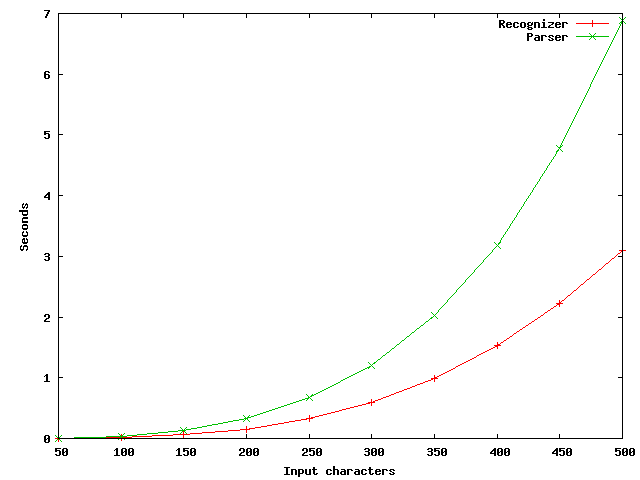
\includegraphics[scale=0.5]{worst-case.png}
\caption{Worst-case recognizer and parser performance scaling.}
\end{figure}

Note however that the recognizer is optimized for speed and the parser for a balance between memory usage and speed (meaning a faster implementation is possible). Regardless of this, it clearly demonstates (close to) cubic worst-case behaviour, as expected (close to, since we can't eliminate JVM interference completely). Looking at the times, our implementation seems very efficient in worst-case scenarios.

\subsection{LL and LR performance}

TODO: Show linear performance on LL and LR grammars.\\
-Using realistic cases would be nice.

\subsection{Grammar factoring}

Apart from worst-case behaviour in terms of the number of ambiguous parse results, it is also interesting to look at how well we perform on worst-case grammars without ambiguous input. Here we will compare the performance of our parser between different version of a grammar; a non-factored version, a left-factored version and a prefix-shared version. The original grammar is the following:\\
$S\,::=\,A+$\\
$A\,::=\,a\,|\,E$\\
$E\,::=\,1\,|\,E\,+\,E\,|\,E\,-\,E\,|\,E\,*\,E\,|\,E\,/\,E\,|\,E\,>\,E\,|\,...$ 25 more like it ...\\
input = $a\,*\,50000$, $a\,*\,100000$, $a\,*\,150000$ and $a\,*\,200000$

It contains lots of left-recursion and one non-ambiguous path. So one would expect non-linear performance in this case. However, as can be seen in the graph below this is not the case. Performance seems to scale perfectly linear regardless of how the grammar is factored.

TODO: Change grammar and text; bottom up (GLR) parsers are likely also linear on this one.

TODO: Highlight differences between different kinds of factoring.

\begin{figure}[H]
\centering
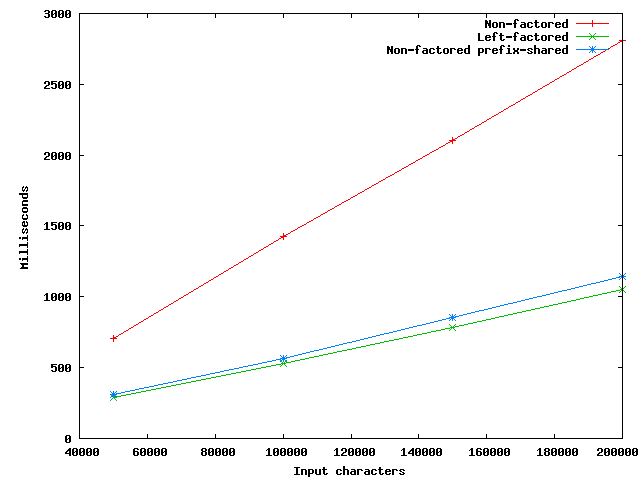
\includegraphics[scale=0.5]{grammar-factoring.png}
\caption{Grammar factoring related parse time scaling; without look-ahead.}
\end{figure}

\section{Prototype}

TODO: Write chapter introduction.

\subsection{Design}

TODO: Write.
-Core.\\
-Stack.\\
--Stack nodes.\\
-Result.\\
--Result nodes.

\subsection{Implementation}

TODO: Write.

\section{Future work}

TODO: Hmm, I'll have to think about this one, I'm kind of done.

\section{Conclusion}

TODO: Write.\\
-Repeat statements from the introduction and acknowledge we proved them.\\
-Damn we're fast.

\section{References}

TODO: Find some, so we can relate it to other stuff. Not basing anything on existing work makes this hard ....

\end{document}
